\documentclass[12pt]{article}
% uncomment the line below if you like. You may lack dependencies if you do.
 \usepackage{proposal}
 \usepackage{float}
 \usepackage{minted}
 \usepackage{subfigure}
 
 
\title{notGuitar - Final Report}
\author{Joey Hall, Paul Chyz, and Jatin Chowdhury}
\date{April 30, 2018}
\begin{document}
\maketitle
\section{Problem Statement}
The main form of instrument conversion in the music industry today is through MIDI conversion. In this process, a note is played on an instrument, software logic determines if a note was played and at which frequency, then the program outputs a recorded sound of a new instrument at the correct note for the desired amount of time. This method works to an extent, but it loses much of the original instrument's dynamic since it is no longer outputting the original signal. 
\newline\newline
Our idea is to use the original signal of an instrument and alter its amplitude and frequency characteristics so that it sounds like a completely new instrument, while still maintaining its dynamics and performing the conversion in real time. We chose to implement this process using a guitar as the original instrument generating the input and making it sound like a saxophone at the output. 

\section{Approach}
The specific sound of a particular instrument is known as the ``timbre'' of the instrument, and is made up two parts: a frequency component and an amplitude component. While most modern audio effects that attempt to change the timbre of one instrument to that of another use MIDI, synthesis, or recorded samples, our approach was to generate the output exclusively by manipulating the amplitude and frequency characteristics of the input signal. The notGuitar system addresses frequency and amplitude characteristics according to the system architecture seen in figure 1.

\begin{figure}[H]
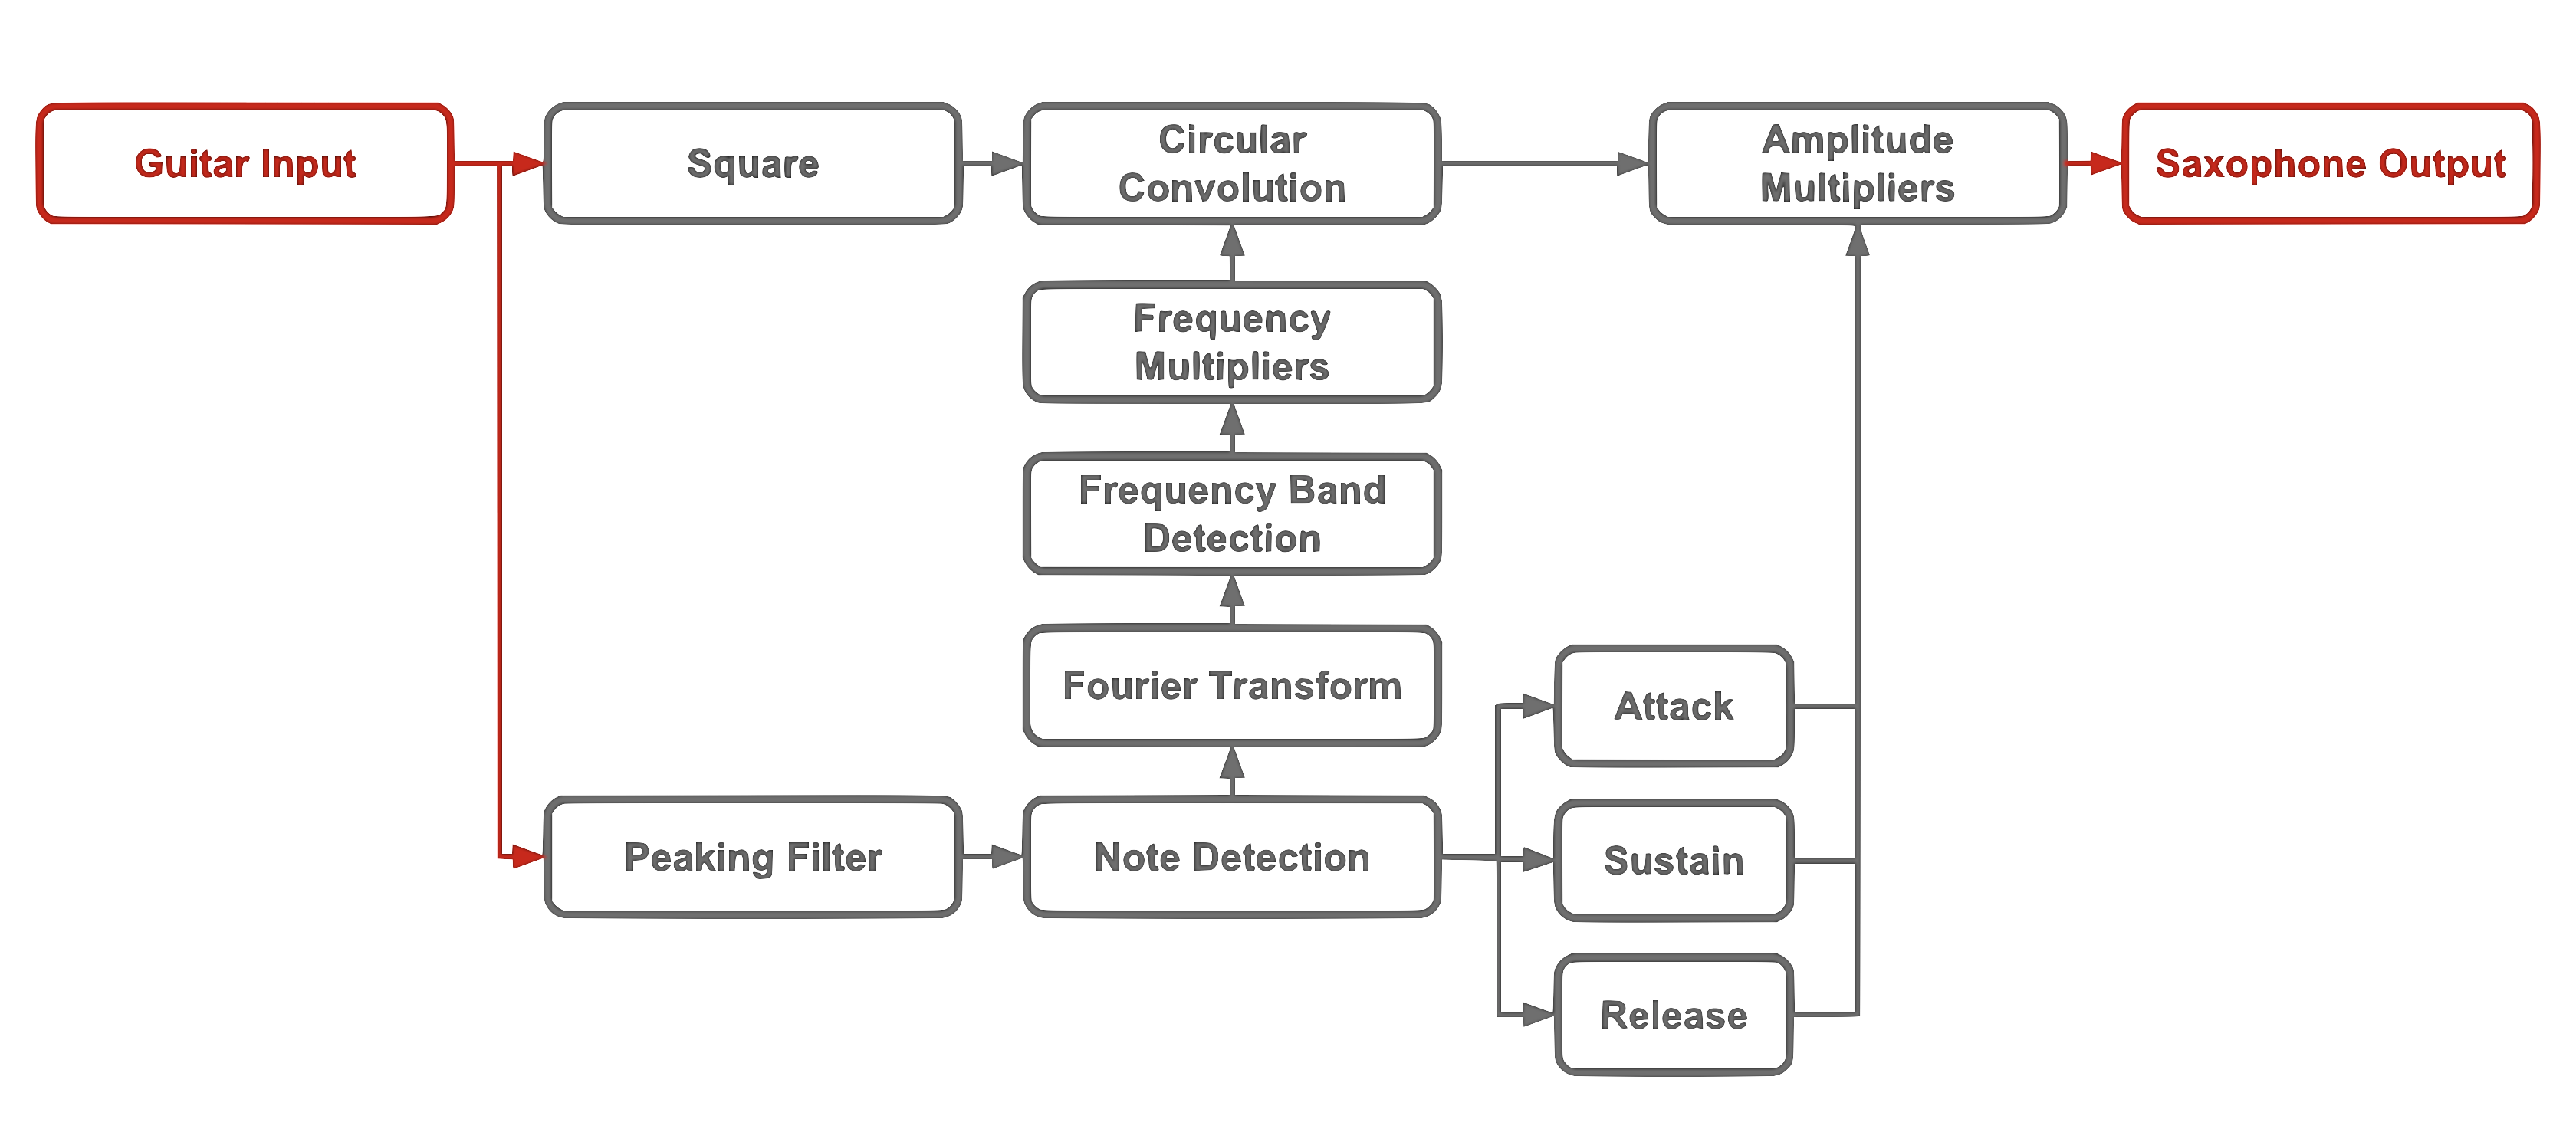
\includegraphics[scale=0.28]{Pictures/FlowChart.png}
\centering
\caption{notGuitar System Flowchart}
\centering
\end{figure}

\section{Frequency Characteristics}
The frequency component of an instrument's timbre is typically referred to as the instrument's ``harmonic structure.'' Essentially, any note played on any instrument produces sound, not just at the fundamental frequency of that note, but also at every multiple of that frequency, known as ``overtones.'' The frequency characteristic of individual instruments exists because the relative amplitude of each harmonic is different for each instrument.
\newline\newline
Our plan for manipulating the frequency content of the signal was to split our frequency spectrum linearly, with enough resolution to isolate individual overtones of any guitar note. We would then use guitar and saxophone sample recordings to train sets of multipliers that could act on the frequency bands to transform the harmonic structure of the guitar to that of the saxophone. Additionally, by detecting a rough band that contained the fundamental frequency, we could tune our multipliers to more accurately represent the harmonic structure relative to the fundamental frequency of the input signal.
\newline\newline
The way that our group approached the frequency component of the guitar to saxophone timbral shift went through many iterations which will be outlines here.
\begin{itemize}
\item Sub-banding Filter Bank:We initially decided to use a linear sub-banding filter bank to split the signal into linearly spaced frequency bands, detect which of the sub-bands contained the fundamental frequency, apply the corresponding set of multipliers, and then sum the signal back together for the output. We abandoned this approach due to the difficulty of summing the sub-bands back together. Since each sub-band would have it's own group delay and phase delay, summing the bands correctly would have been non-trivial.

\item Short Time Fourier Transform: Our next plan was to use a Short Time Fourier Transform (STFT) to represent split up the frequency spectrum. Since an N-window Fourier Transform essentially splits the positive frequencies into N linearly spaced frequency bins, we could use the STFT to find the fundamental frequency, and apply the multipliers, and then to sum the bins back together, we would only need to take the inverse STFT. While this method was well suited for our purposes, we ended up abandoning the STFT because of its increased time complexity relative to methods that we later found.

\item Sliding Discrete Fourier Transform: Since the STFT described above would be operating on the same window in consecutive time steps, except for one new sample entering the window, and one old sample leaving the window, we next considered using a Sliding Discrete Fourier Transform (SDFT) in place of the STFT \cite{SDFT}. While STFT has a time complexity of $\mathcal{O}(n\log{}n)$ for both the forward and inverse transform, the SDFT is $\mathcal{O}(n)$ for the forward transform. That said, computing the inverse DFT in a similarly recursive manner proved to be more difficult, and by the time we had figured out a way to do it, we had replaced the SDFT with a circular convolution altogether. However, in the final system, the SDFT is used to calculate the Fourier transform of the first four frequency bins, which then informs the system which set of frequency multipliers to use for the circular convolution.

\item Circular Convolution: Since the multiplication of two signals in the frequency domain corresponds to the convolution of those signals in the time domain, we ultimately decided to perform the frequency effect of our system using a circular convolution, which proved to be the optimally efficient method. The SDFT needed N complex-by-complex multiplications for the forward transform, and $\frac{N}{2}$ real-by-complex multiplications for the inverse transform, plus an additional N real-by-complex multiplications for the frequency multipliers, the total time complexity of the system with the SDFT would have been $\mathcal{O}(7n)$. By contrast, the circular convolution had a total time complexity of $\mathcal{O}(n)$.
\newline\newline\newline
\end{itemize}

\subsection{Frequency Multipliers}
After gaining the ability to manipulate the frequency content of the input signal with circular convolution, we needed to generate the overtone weightings to properly convert a guitar's harmonic structure into one that matches a saxophone. To do this, we recorded 25 notes on both guitar and saxophone, and used Matlab to detect the relative amplitudes of each overtone for all the notes. These relative amplitudes allowed us to calculate a multiplier value to be applied to each overtone, imposing the frequency characteristics of a saxophone on the guitar signal. However, our implementation of these frequency multipliers needed to address limitations in frequency resolution, high frequency content, and circular convolution adaptations.
\begin{itemize}
\item Frequency Resolution: Due to the system using circular convolution to split the frequency spectrum linearly, there were inherent limits on the width of each resulting frequency bin. In order to maintain an acceptable resolution for the frequency multipliers, we designed the convolution to produce frequency bins that are 128 Hz wide. This width corresponds to the frequency spacing of the overtones for the lowest note in our training system. As the input signal increases in frequency from that note, the overtone spacing will increase, and the effective resolution of the system will improve from its baseline accuracy. This fixed bin width also required a change from our initial plan to isolate each overtone. Instead, we generated one set of frequency multipliers for each frequency bin, averaged from the training notes with fundamental frequencies in each given bin. These averaged multipliers contained between 5 and 12 notes per frequency bin, along with a set of multipliers generated from the average of all 25 notes.

\item High Frequency Content: During our frequency multiplier testing, we found that the guitar input samples contained fewer high frequencies than the saxophone samples we were trying to replicate. Our problem statement included a focus on avoiding any synthesis or sampling, so we had to work out a way to generate more high frequency content from the input signal itself. After trying methods of summing the signal and its square and summing the signal with a copy that was modulated by a cosine, we settled on using the input signal summed with a scaled square of the same signal. The scaling allowed us to control the intensity of the high frequencies from the square relative to the lower frequencies that were already present. By training with this modified signal and performing the same operation on the input signal in our real-time system, we were able to generate enough high frequency content and weight it appropriately to match the harmonic structure of a saxophone.

\item Circular Convolution Adaptations: Once the frequency multipliers were generated, they had to be adapted for implementation with circular convolution. The matlab training algorithm worked in the frequency domain, but the multiplier values needed to work in the time domain in the real-time system. To make this adjustment, we took the inverse DFT of the multiplier values, allowing them to be applied to the guitar input signal with circular convolution. In real-time, this system applies the 25-note average multiplier to the input signal until it can determine which frequency bin contains the current fundamental, at which point it applies the corresponding frequency bin average multipliers.

\end{itemize}

\subsection{Simulations}

\begin{figure}[H]
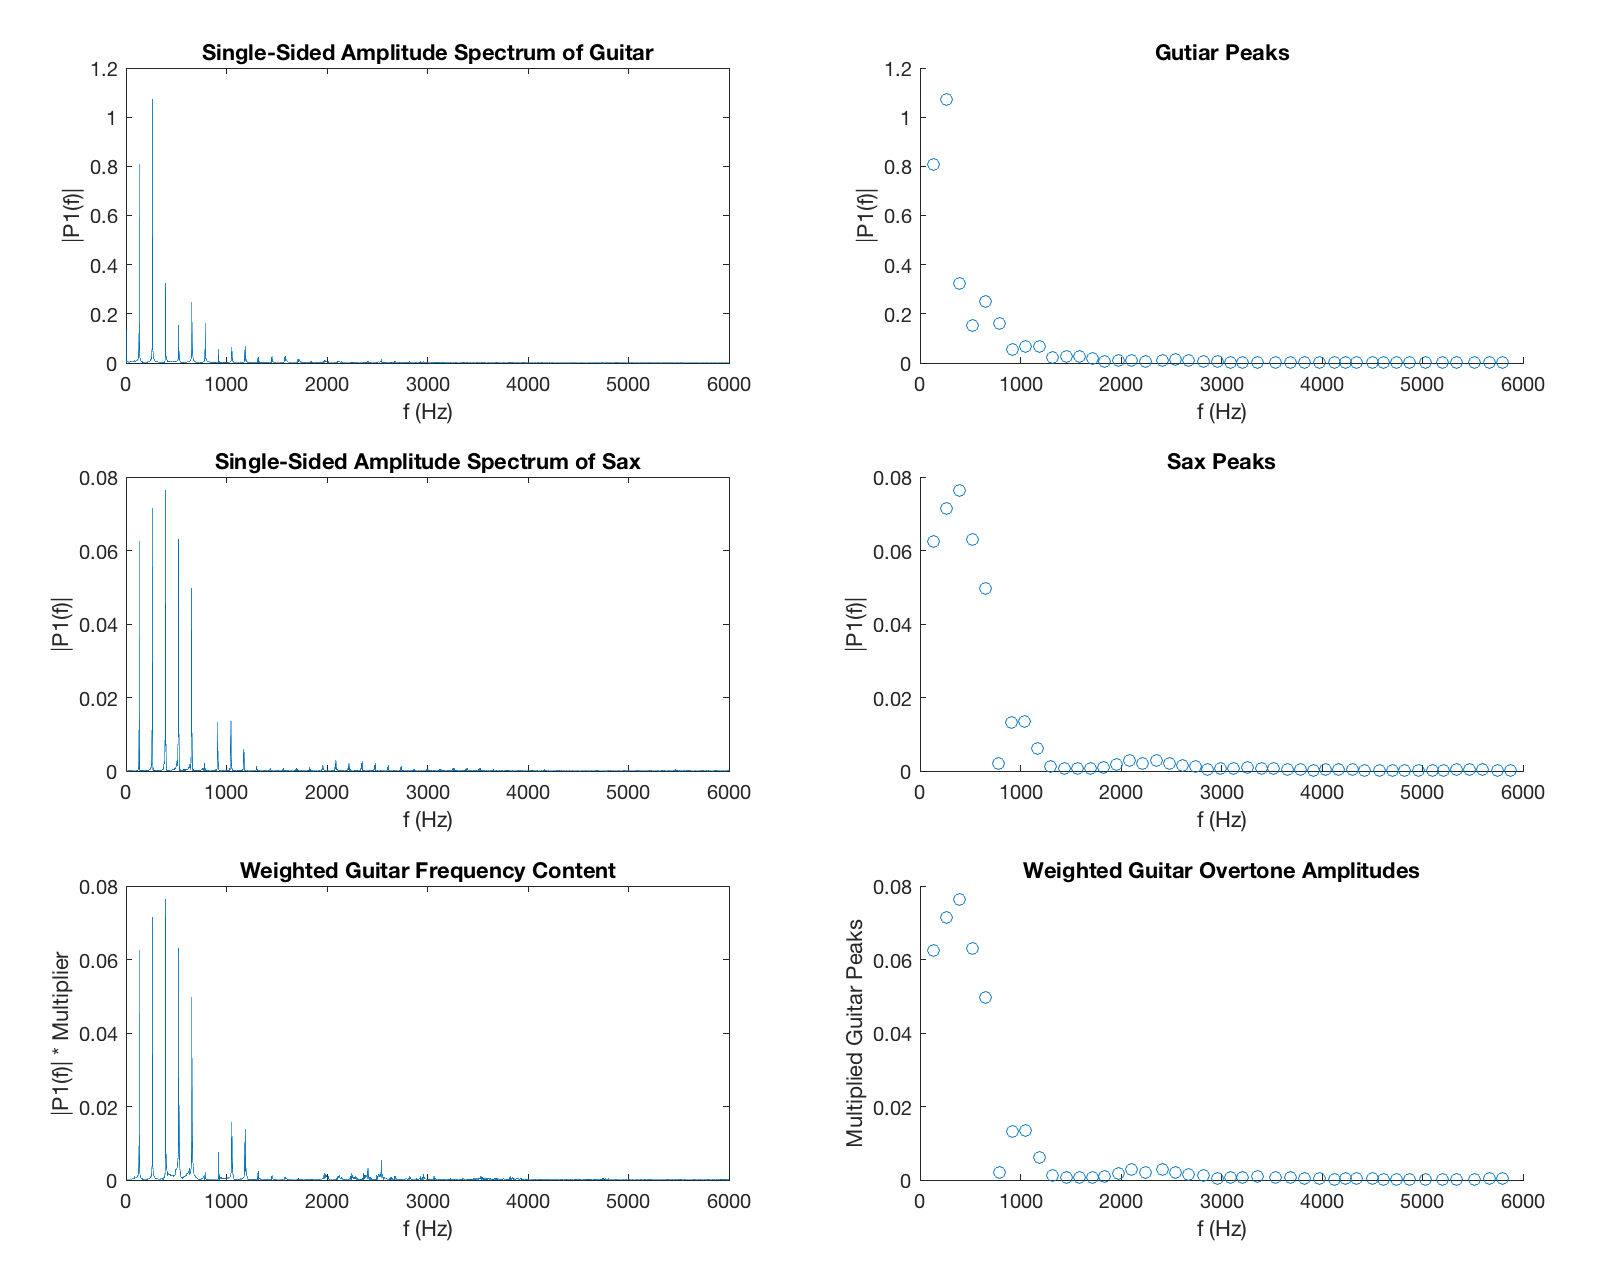
\includegraphics[scale=0.3]{Pictures/FreqPlot1.png}
\centering
\caption{Overtone Amplitude Detection and Simulation of Applied Multipliers}
\centering
\end{figure}

\begin{figure}[h]
\subfigure{
  \centering
  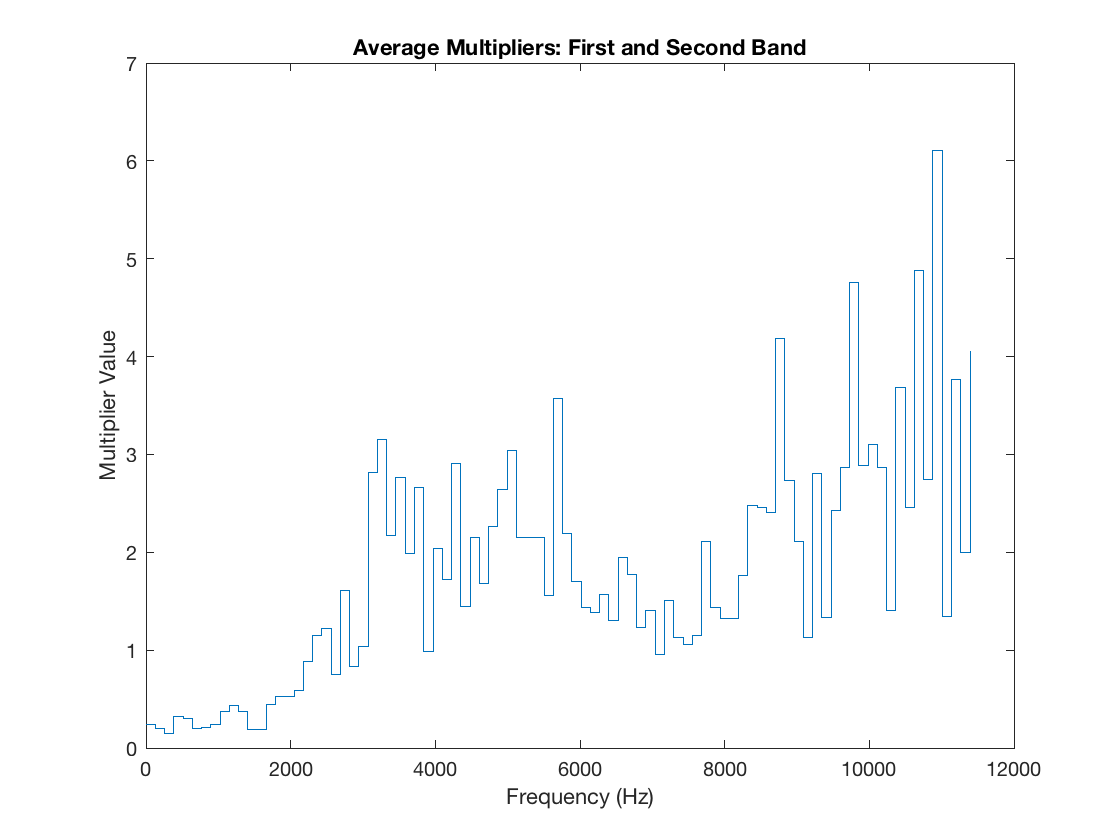
\includegraphics[width=.47\textwidth]{Pictures/FreqMult1_2.png}
}
\subfigure{
  \centering
  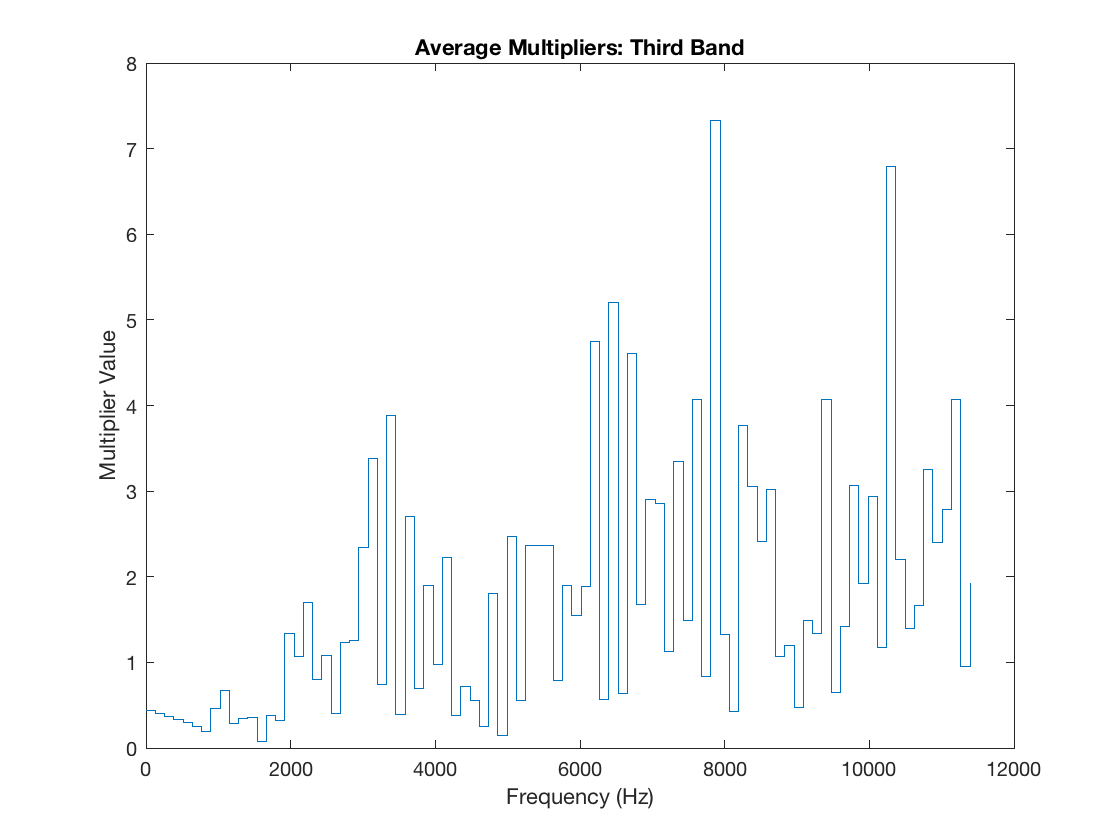
\includegraphics[width=.47\textwidth]{Pictures/FreqMult3.png}
}
\caption{Frequency Multipliers for the first and second frequency bin (left) and for the third frequency bin (right)}
\centering
\end{figure}

\begin{figure}[h]
\subfigure{
  \centering
  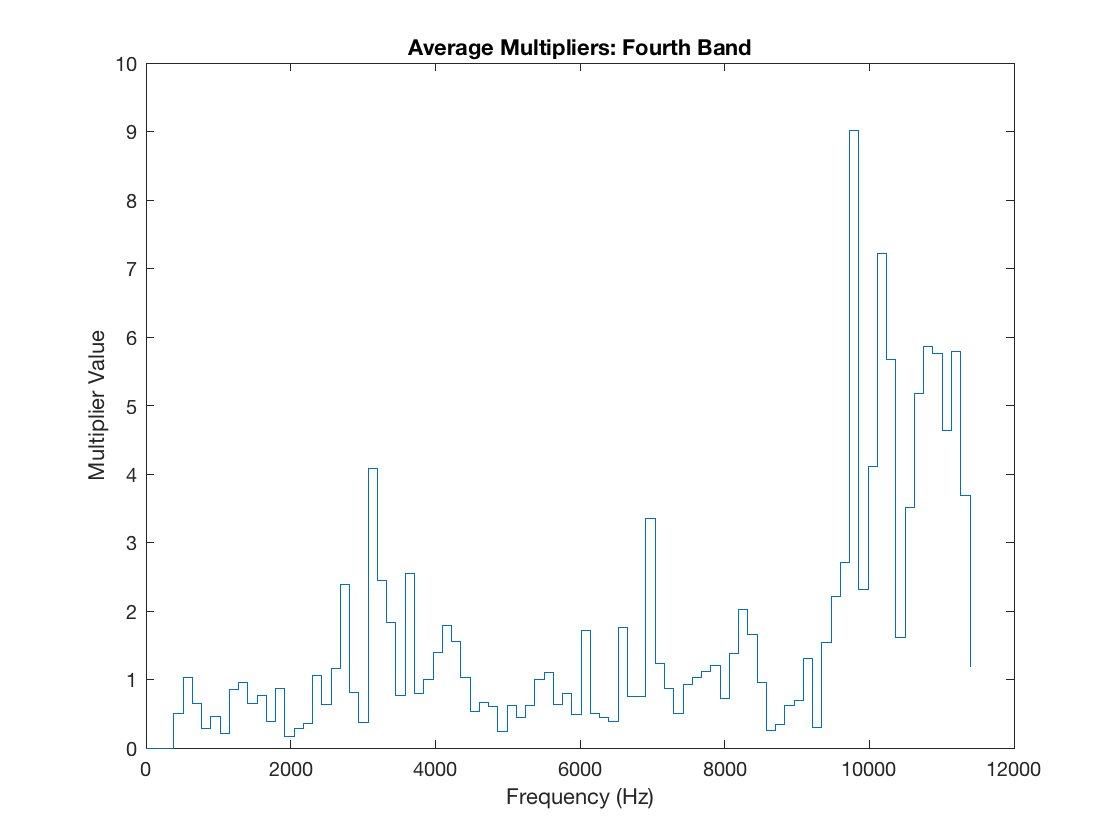
\includegraphics[width=.47\textwidth]{Pictures/FreqMult4.png}
}
\subfigure{
  \centering
  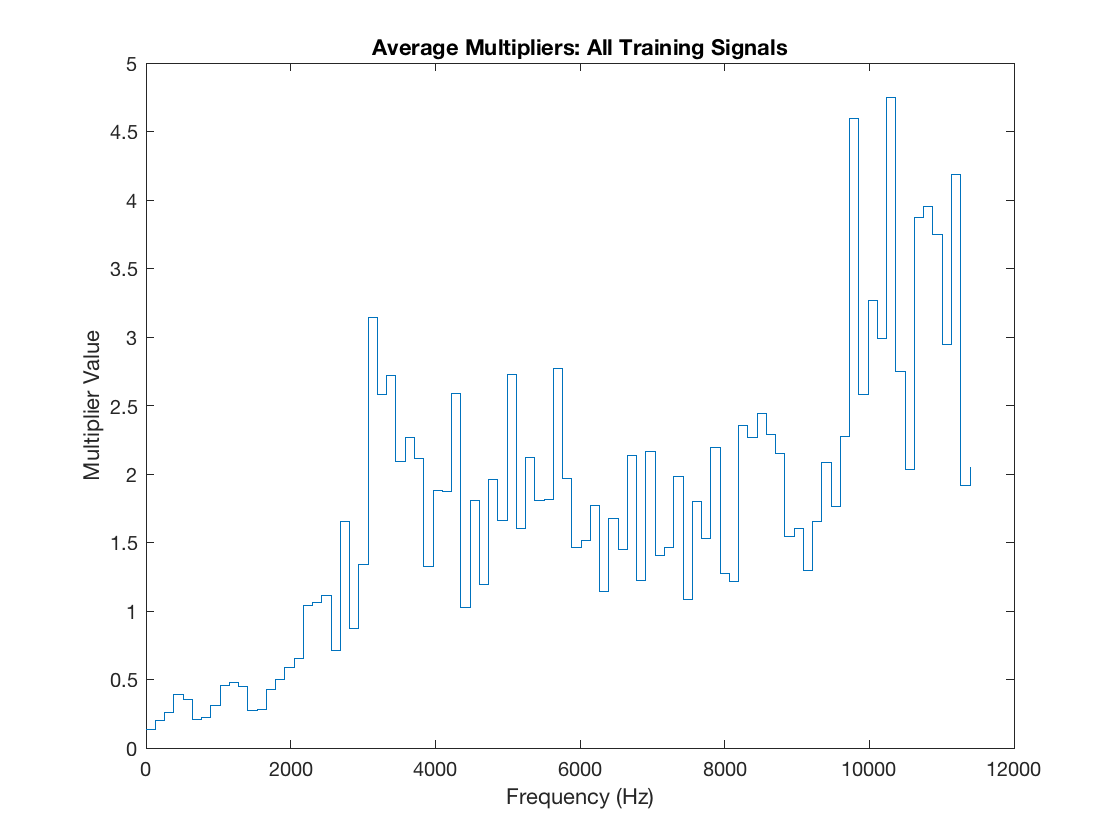
\includegraphics[width=.47\textwidth]{Pictures/FreqMultAll.png}
}
\caption{Frequency Multipliers for the fourth frequency bin (left) and for all training signals (right)}
\centering
\end{figure}


\subsection {Results}
This overtone manipulation task was a difficult one in practice due to the constraints in resolution and in frequency content. Given the limitations, this system performs well, and the output signal has a very different sound that comes fairly close to that of a saxophone. The lack of high frequency content in the guitar input signal made it difficult to produce a fully natural sound, as the square of the input signal introduced high frequency noise and distortion that seemed to distract from the intended sound. When paired with the amplitude manipulation, the output becomes much less associable with a guitar, and depending on the user's playing style, it can contain characteristics that sound surprisingly similar to a saxophone. 
\newline\newline
Some improvements that could be made to this system before producing a marketable product include more rigorous training, optimization of frequency bin widths and average multipliers, and sample rate improvements. Training the multipliers with multiple versions of each note from different guitars would produce a more robust system that would sound better for a wider range of use cases. Similarly, optimizing the system to increase the frequency resolution would allow for more isolated overtone multipliers. This in turn would improve the effectiveness of the averaged multipliers. Finally, increasing the sample rate to 44.1 kHz would not only reach the industry standard for audio technology, but it would allow some of the noise and distortion from the squared signal to be separated from the input signal due to the increased frequency spectrum before the Nyquist frequency.

\color{black}
\section{Amplitude Characteristics}
Along with a unique harmonic structure, each musical instrument also has a unique amplitude envelope. The combination of amplitude envelope and harmonic structure are theoretically what define the complete timbre of an instrument.  The amplitude envelope has three parts, the attack, sustain and release. 

\begin{figure}[H]
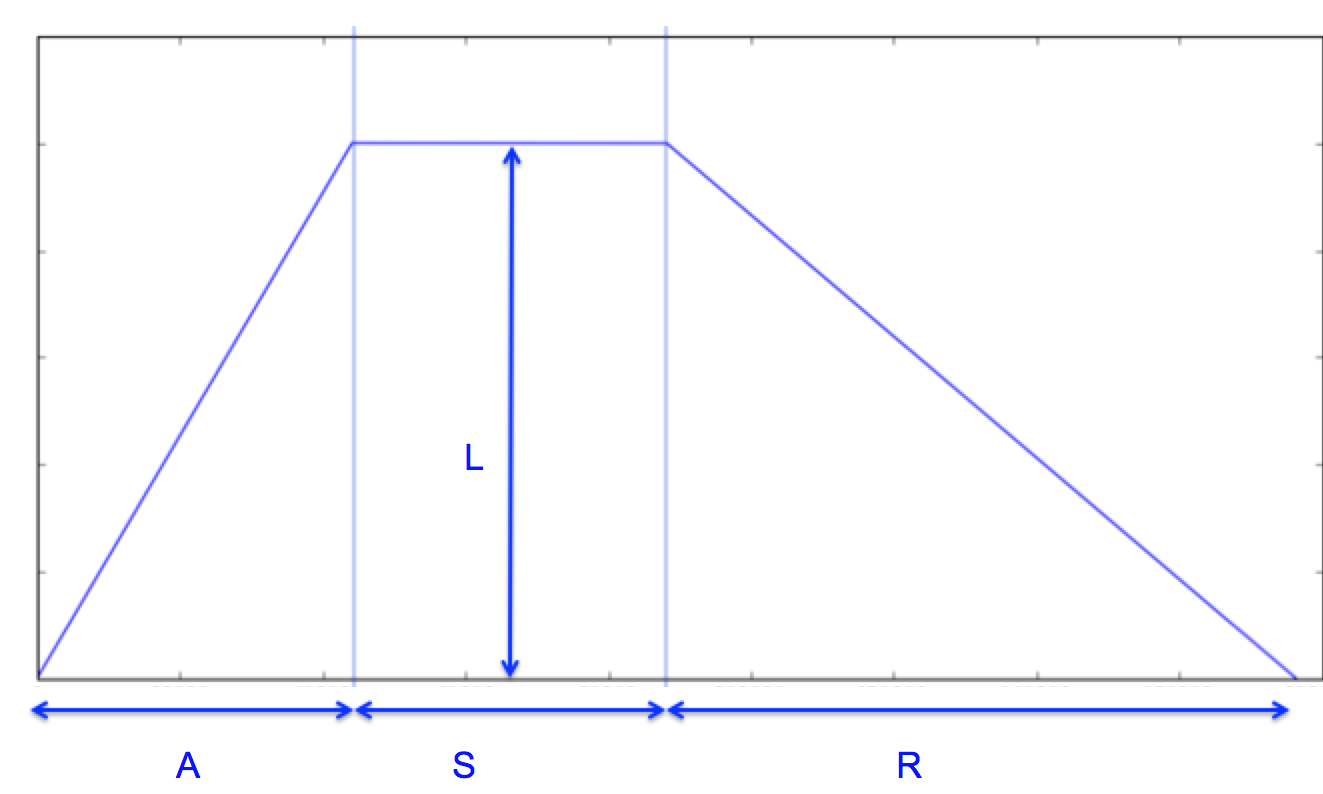
\includegraphics[scale=0.5]{Pictures/ASR.png}
\centering
\caption{The ASR Amplitude Envelope}
\centering
\end{figure}

\begin{itemize}
\item Attack: The attack of a note is essentially the event that triggers the onset of the note. For example, the attack of a saxophone would be the sound of the pick hitting the string, while the attack of a saxophone would be the sound of the tongue hitting the reed.
\item Sustain: The sustain of a sound characterizes the way that the amplitude of a note changes as it is held out. For a guitar, the amplitude decays as the vibration energy of the string gradually diminishes. For the saxophone, however, the amplitude during the sustain stays roughly constant as the saxophone player uses their breath support to maintain the volume of the note.
\item Release: Just as the attack is the event that triggers the onset of the note, the release is the corresponding event that turns the note ``off.'' For the saxophone the release is triggered by the player choking of their air, while the release of the guitar can be heard as the sound of the player's fingers muting the strings.
\end{itemize}
\noindent
The way we approached the amplitude aspect of converting from the timbre of a guitar to that of a saxophone was to use note detection methods to determine which part of the amplitude envelope the input signal was in, and then use multiplier tables to scale the signal to match the amplitude envelope of the saxophone.

\subsection{Envelope Detection}
In order to generate the amplitude multiplier tables mentioned above, it was first necessary to analyze saxophone and guitar samples off-line to characterize the natural amplitude envelopes of each instrument. We implemented an envelope detection method as described in \cite{DBLP:journals/corr/Jarne17} which consists of rectification followed by a peaking filter followed by a low pass filter. We were then able to store the envelope values for the attack and release parts of the waveform to be used in real-time (see Figure 7).

\begin{figure}[h]
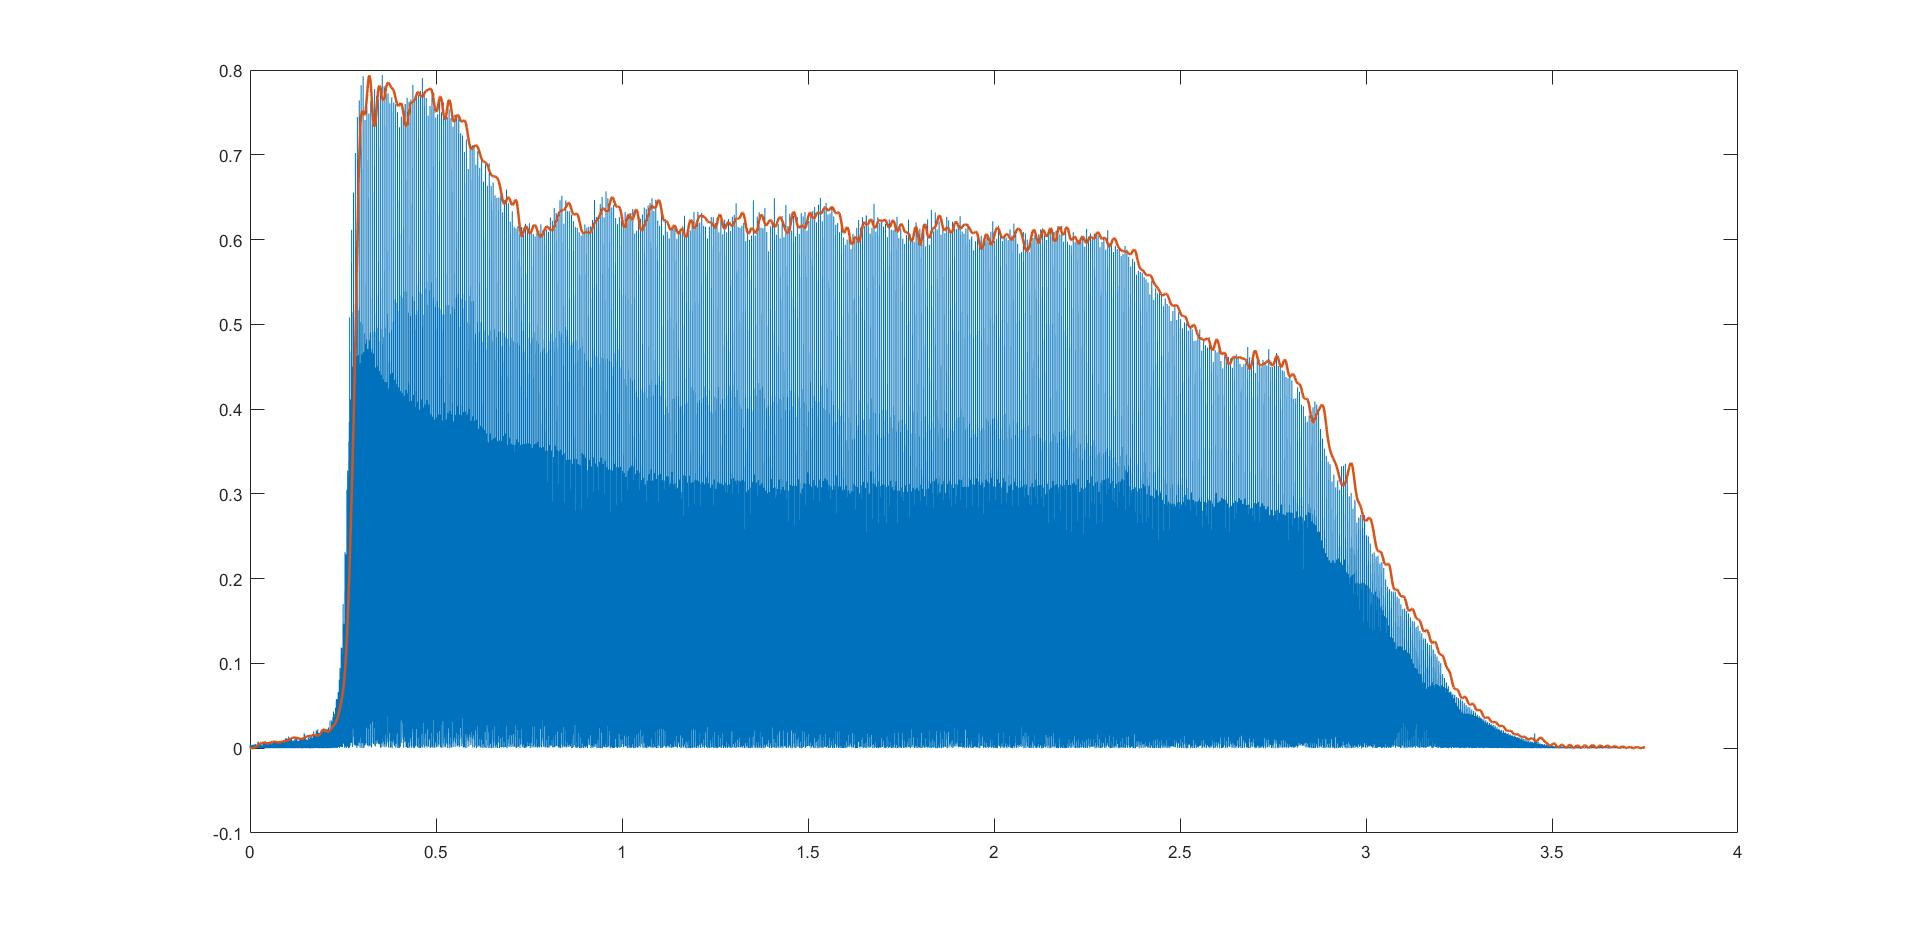
\includegraphics[scale=0.2]{Pictures/EnvDetection.jpg}
\centering
\caption{Envelope Detection for Saxophone Sample}
\centering
\end{figure}
\setlength{\abovecaptionskip}{-20pt}
\begin{figure}[h]
\subfigure{
  \centering
  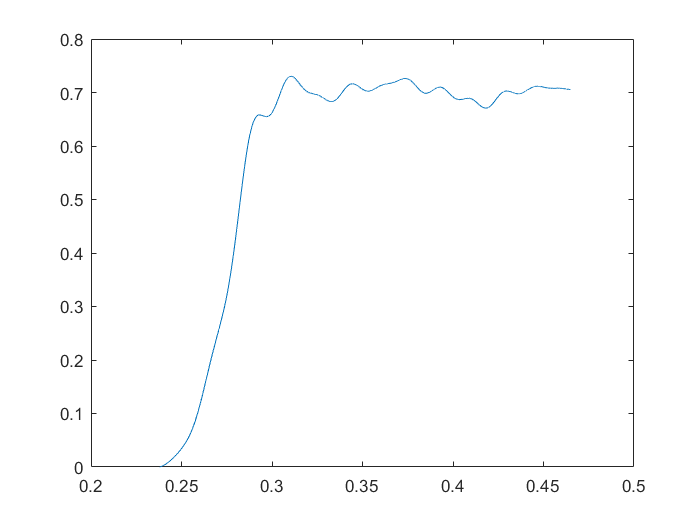
\includegraphics[width=.5\textwidth]{Pictures/Attack_Env.png}
}
\subfigure{
  \centering
  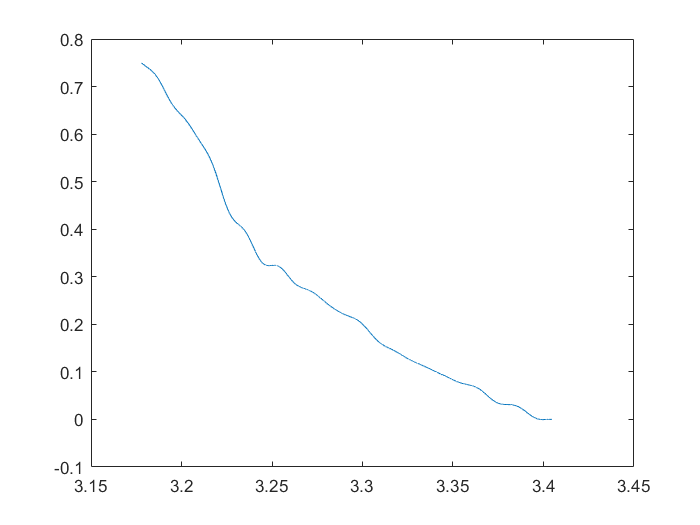
\includegraphics[width=.5\textwidth]{Pictures/Release_Env.png}
}
\caption{Attack and Release Multipliers}
\end{figure}

\subsection{Note Detection}
In order to implement the envelope modulation, it is necessary to detect the onset and offset of every note, and use those to trigger the attack and release multipliers. Following the process outline in \cite{NoteOnset} we first implemented a short window peaking filter, and then used a threshold to determine when a new note had begun (see Figure 8). Using the same method, but with a different threshold, we were able to detect the ends of notes as well. The issue with this method, was that if a note was already being sustained while the next note was played, the algorithm would not be able to detect the onset of the new note. To remedy this, we added another method of note detection: during the sustain part of the waveform, if the output of the peaking filter was some threshold above the average of the peaking filter window, we consider that a new note, and thus trigger the attack envelope modulation.
\setlength{\abovecaptionskip}{5pt}
\begin{figure}[h]
\subfigure{
  \centering
  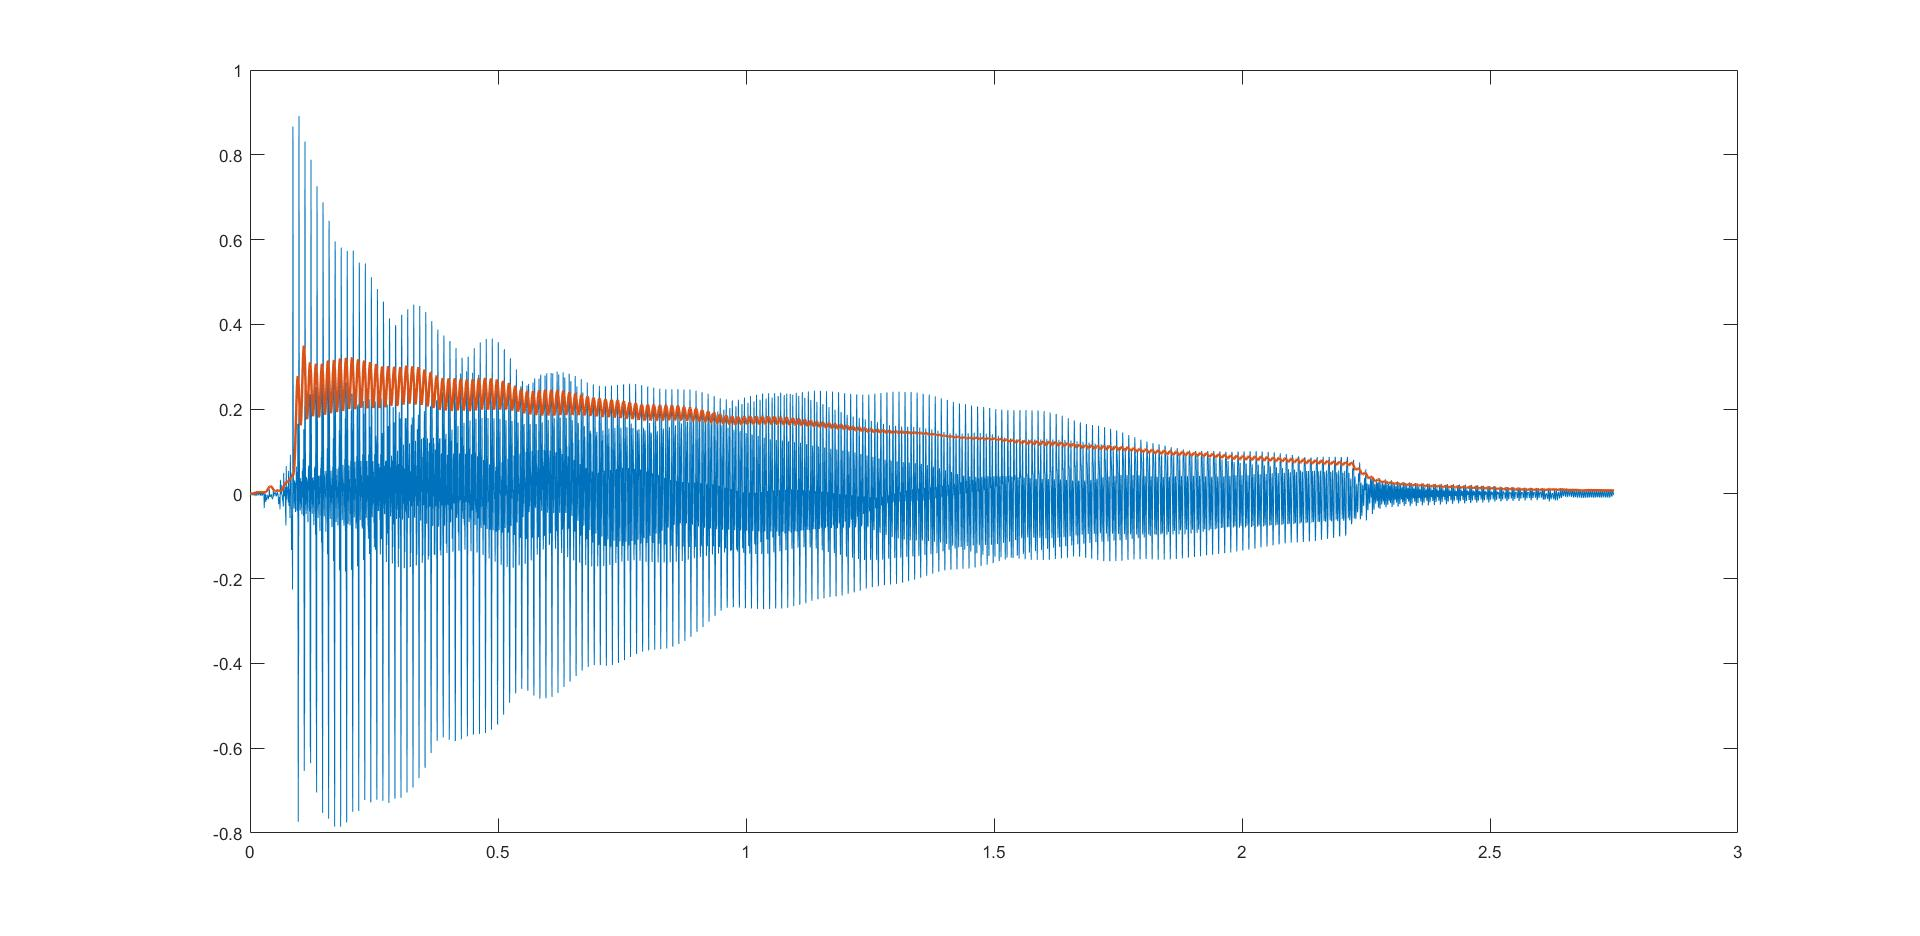
\includegraphics[width=.47\textwidth]{Pictures/NoteDetect1.jpg}
}
\subfigure{
  \centering
  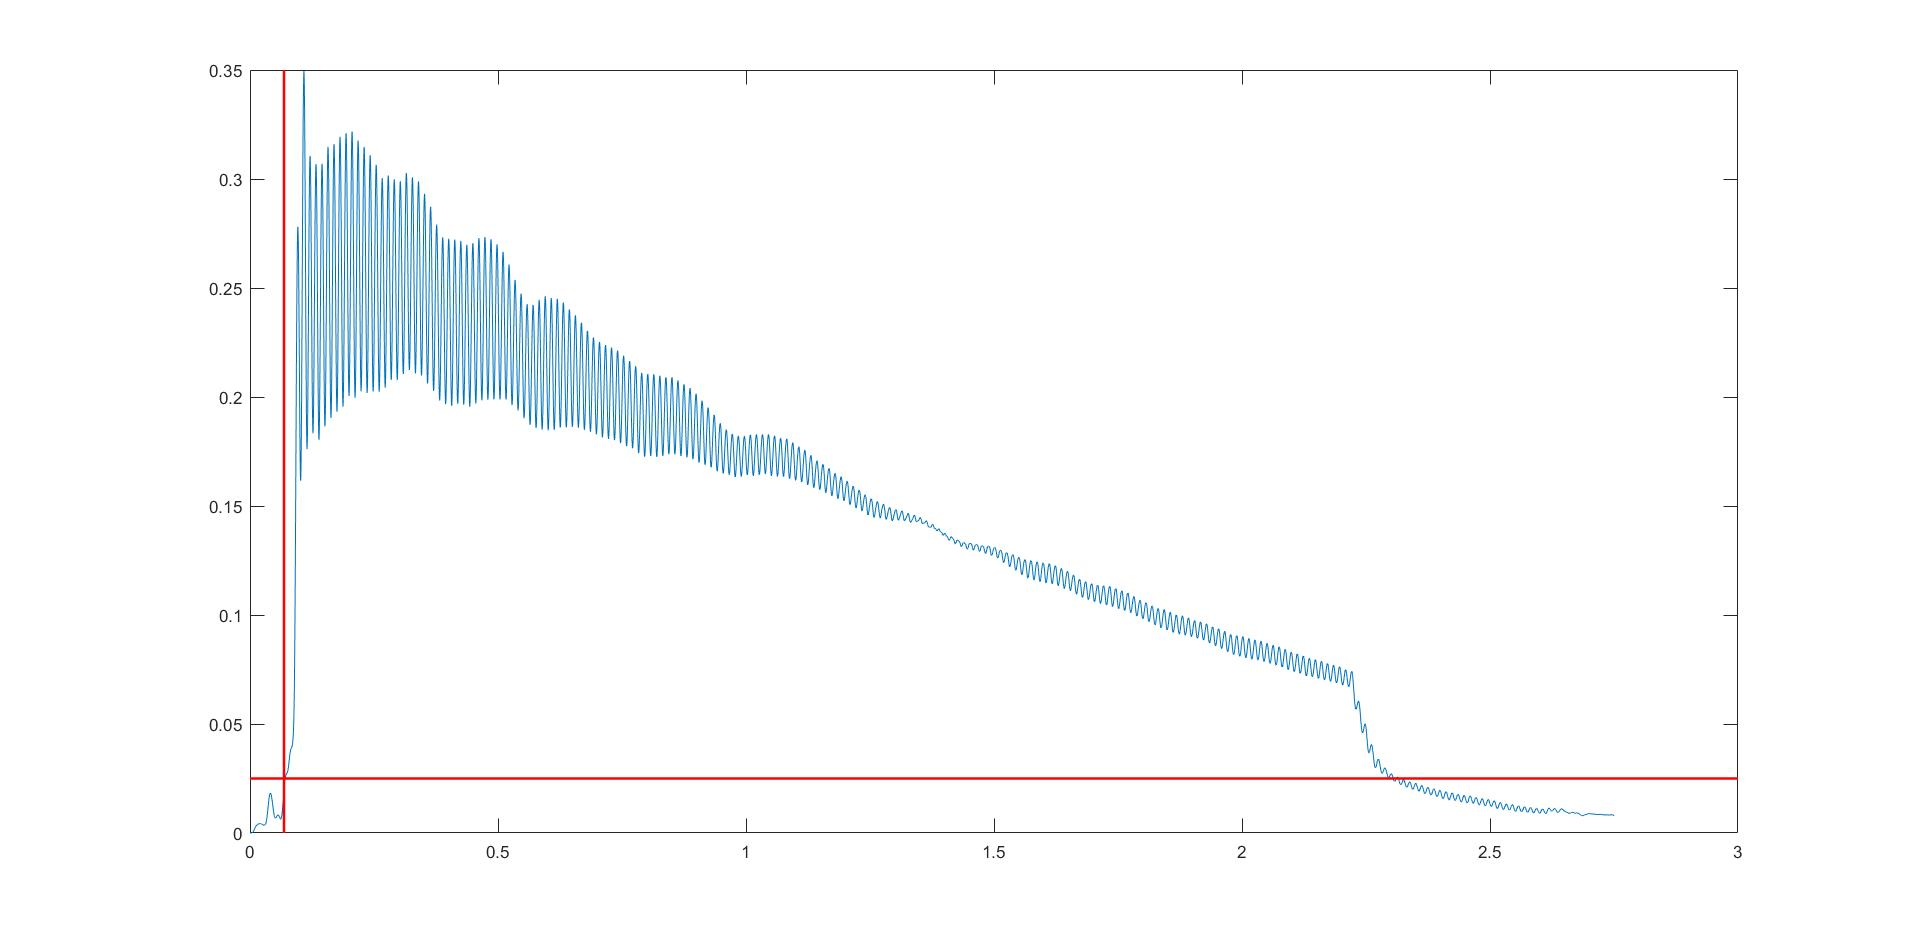
\includegraphics[width=.47\textwidth]{Pictures/NoteDetect2.jpg}
}
\caption{Note Onset Detection for Guitar Sample}
\centering
\end{figure}

\subsection{Sustain}
Finding a transfer function for the sustain part of the waveform proved to be somewhat more difficult, because unlike the attack and release, the sustain can last for an indeterminate amount of time - as long as the player holds the note. As such, our sustain transfer function needed to be able to operate over an arbitrarily long signal without losing stability. In order to meet these demands, we model the guitar sustain as an exponential decay, and the saxophone sustain as being roughly flat. Therefore, in order to obtain the flat response from the exponential decay, we need to multiply the signal by an exponentially increasing function (see Figure 9). Along with giving our sound a much more saxophone-like sustain, the advantage of modeling the sustain in this way, is that as the sustain extends to be arbitrarily long, the transfer function approaches a constant multiplier value, thus ensuring stability.

\begin{figure}[H]
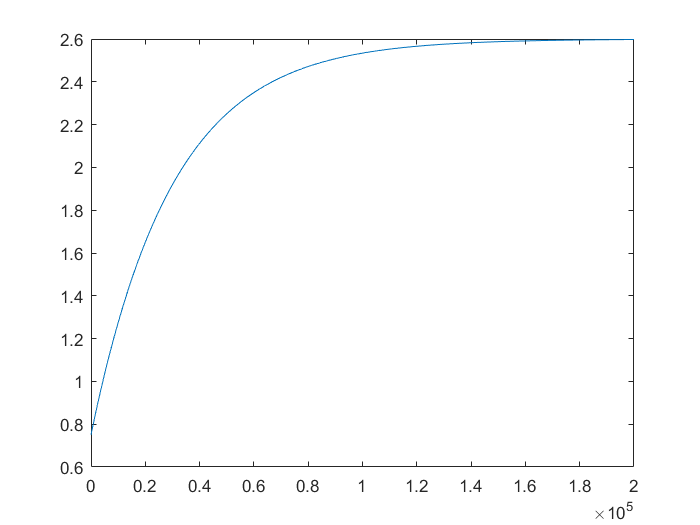
\includegraphics[scale=0.55]{Pictures/Sustain_Env.png}
\centering
\caption{Sustain Envelope}
\centering
\end{figure}

\subsection {Results}
Ultimately, the amplitude envelopes worked as expected for all three parts of the waveform,  creating the smooth attack that listeners expect from the saxophone, and maintaining a roughly flat sustain without robbing the sound of its human quality as a MIDI system would do. The note detection algorithm worked reasonably well for single notes, but even with the enhanced note detection scheme described above, had difficulty detecting every new note in a multi-note melody, particularly if notes were played very quickly in succession. The result was a slightly ``choppy'' sound that we would need to improve in order to commercialize a system such as this one. An additional improvement would be to make the threshold values more robust, perhaps by comparing to a noise floor, rather than simply using hard-coded values. Below, we see input and output waveforms of a single guitar note passed through a DSP board running the algorithm in real-time.

\setlength{\belowcaptionskip}{5pt}
\begin{figure}[H]
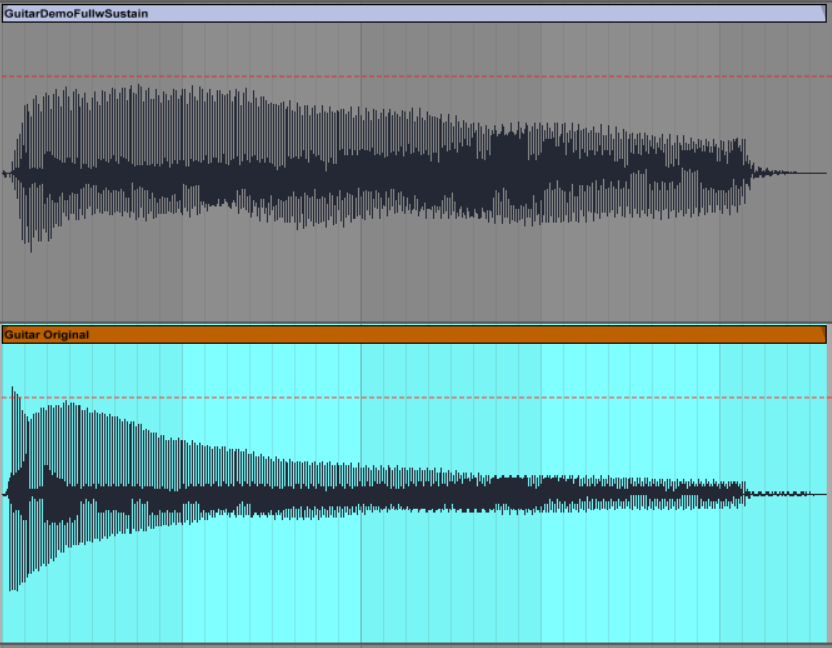
\includegraphics[scale=0.6]{Pictures/Final_pic.PNG}
\centering
\caption{Amplitude Envelope Results: Guitar Input (below), notGuitar Output (above)}
\centering
\end{figure}

\section{Future Improvements}
Currently using the DSK6713, our system is too large to be attractive to the average consumer; ideally it would need to be the size of a standard guitar effects pedal (3x5x2 inches). The system would also benefit from having faster hardware so that we could run the board at 44.1 kHz instead of 24 kHz. 44.1 kHz is industry standard and would allow the system to account for all frequencies in the human hearing range. To get to these improvements we would either need to have a more modern DSP board or have a custom integrated circuit built to perform these functions efficiently.
\newline\newline
Our system is also only trained to be used for one note at a time, which limits the amount of things that a guitar player can do with it. Even though saxophones technically cannot play chords, implementing a feature where the user can play a chord and have it sound like several saxophones playing different notes of the chord at the same time would be a very useful feature. However, this feature would require a multi-note frequency detection algorithm, which will take more computation power.
\newline\newline
In order to add more variety to the project and appeal to a broader audience, we would like to have this system work not only for guitar to saxophone, but for any instrument as both the input and the output. Examples would include trumpet, violin, flute, etc.. This would require more off-line training to identify the frequency and ampliture characteristics of each instrument, but would be very doable. Another aspect that would enhance the user experience would be to have the pedal be adaptable for users' desired control. The system could allow for the user to vary the timbre intensity and/or have a foot pedal for sustain length.

\section{Documentation of Real-Time System}
A video demonstration of the notGuitar system working in real-time can be found here: \url{https://www.youtube.com/watch?v=0Gk7cZHvSLI&feature=youtu.be}.


\bibliographystyle{unsrt}
\bibliography{references}

\end{document}
